%\documentclass[pdf,notes]{beamer}
\documentclass[pdf,handout]{beamer}
\mode<presentation>{\usetheme[secheader]{Boadilla}}
\usepackage{mystyle}
\includecomment{versiona}
\usepackage{xeCJK}
\usepackage{subfig}

%\setbeameroption{hide notes}
\newcommand{\red}[1]{{\color[rgb]{0.6,0,0}#1}}
\setCJKmainfont[AutoFakeBold=true]{Hiragino Mincho Pro} %my Mac
%\setCJKmainfont{MS PGothic} %AJP windows

\makeatletter
\newenvironment<>{proofs}[1][\proofname]{\par\def\insertproofname{#1\@addpunct{.}}\usebeamertemplate{proof begin}#2}
{\usebeamertemplate{proof end}}
\makeatother

\makeatletter
\def\th@mystyle{%
\normalfont % body font
\setbeamercolor{block title example}{bg=orange,fg=white}
\setbeamercolor{block body example}{bg=orange!20,fg=black}
\def\inserttheoremblockenv{exampleblock}
}
\makeatother

\theoremstyle{mystyle}
\newtheorem{prop}{Proposition}

\title{Hermitian Neural Networks}
\subtitle{joint with 小林俊行}
\author{レオンチエフ・アレックス、東大数理}

\begin{document}
\begin{frame}\titlepage\end{frame}
\begin{frame}{Outline}
\tableofcontents
\end{frame}
\newcommand{\mytime}[1]{(#1{分})}
\section{Intro: Orthogonal Neural Networks}
\begin{frame}
	\begin{figure}[h]
		\centering
		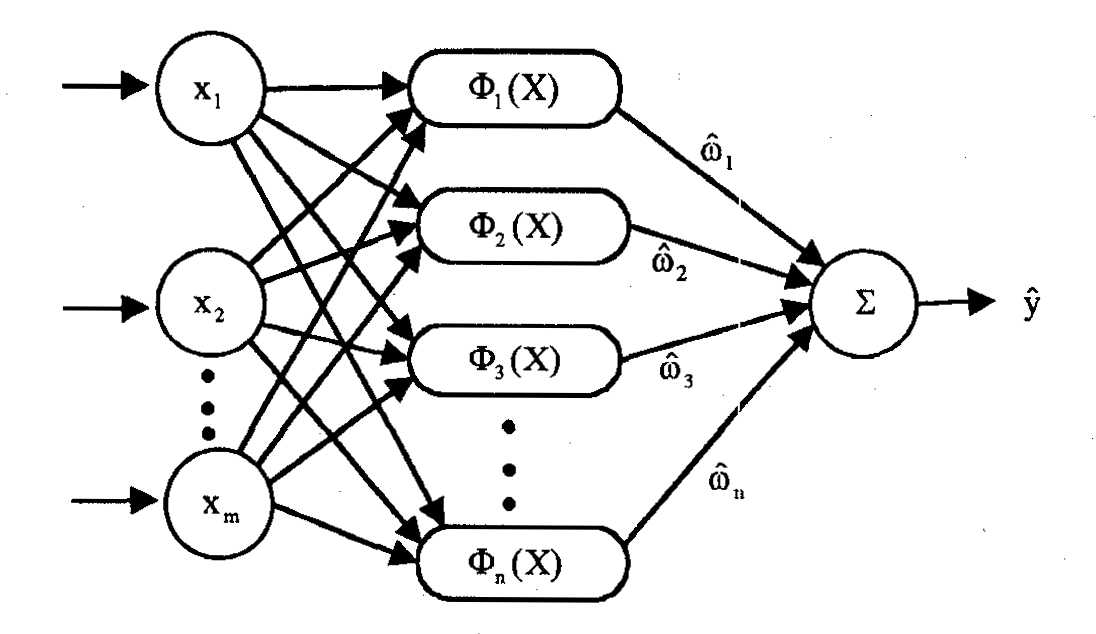
\includegraphics[scale=0.3]{onn}
		\caption{Orthogonal Neural Network (taken from \cite{yang1996orthogonal})}
		\label{fig:onn}
		%\note{tesime}
	\end{figure}
	\begin{block}{Idea}
		Approximate signal $y(x)$ using orthogonal functions:\begin{equation*}
			y(x)\approx \hat{y}(x):=\sum_{i=1}^N \hat{\omega}_i  \Phi_i(x)
		\end{equation*}
	\end{block}
	This connects neural networks with functional analysis!
\end{frame}
\begin{frame}{Advantages}
	\begin{itemize}
		\item Architecture is simple;\pause
		\item Parameters are few;\pause
		\item Can choose particular OFs to suit the particular problem domain (e.g.  Hermitian for medical imaging);\pause
		\item Error estimation is readily available ($\implies$ can estimate convergence speed);\pause
		\item For some OFs we can use recurrence relations to speed up the computation (e.g. Lagrange, Hermitian)
	\end{itemize}
\begin{figure}
  \centering
  \vspace{-0.6cm}
  \subfloat{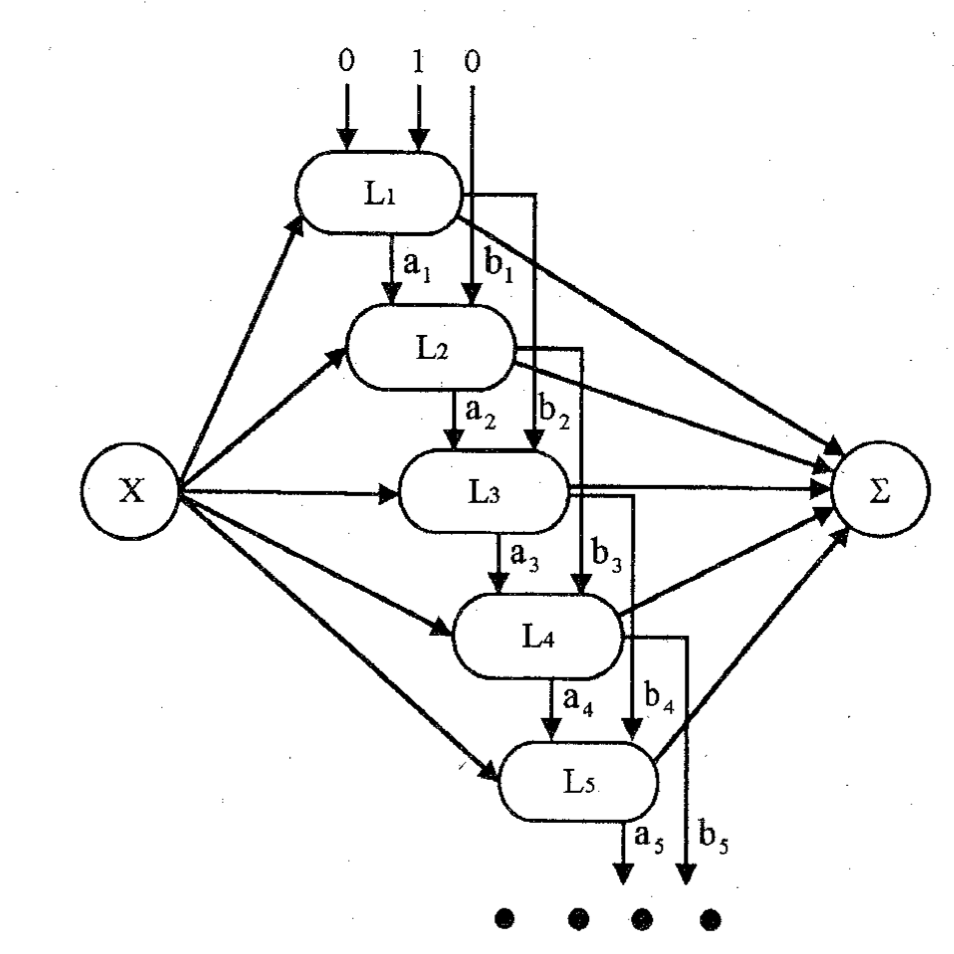
\includegraphics[scale=0.2]{onn2}}\qquad
  \subfloat{\raisebox{0.5cm}{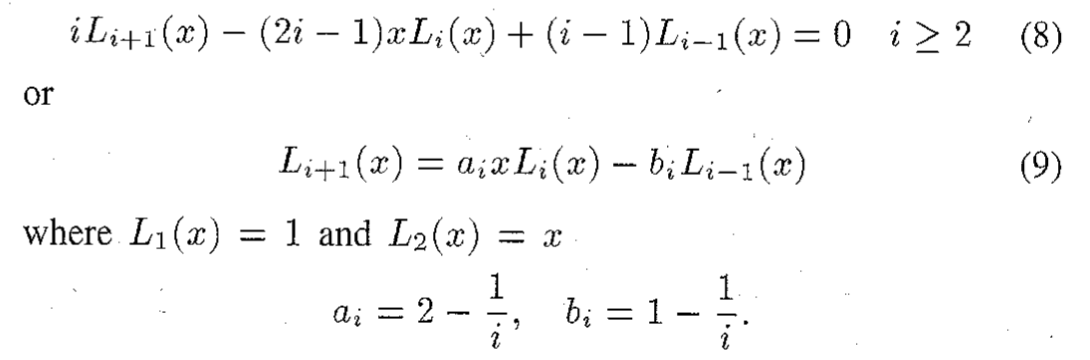
\includegraphics[scale=0.4]{onn3}}}
\caption{(taken from \cite{yang1996orthogonal})}
\end{figure}
\end{frame}
\section{Intro: Convolution of Hermitian Neural Networks}
\begin{frame}{Why Hermitian Networks}
	\begin{equation*}
		\begin{array}[]{c}
		h_n(t)=\frac{H_n(t)e^{-t^2/2}}{\sqrt{2^nn!\sqrt{\pi}}}\\
		H_n(t)=(-1)^n e^{t^2}\frac{d^n}{dx^n}e^{-x^2}
		\end{array}
	\end{equation*}
	\begin{itemize}
		\item Low order 
	\end{itemize}
\end{frame}
\section{Intro: Hermite-Rodriguez Networks}
\section{My contribution}
\section{Further work}
\section{Q\&{A}\mytime{20}}
\begin{frame}
	\begin{center}
		\Huge Q\&{A}
	\end{center}
\end{frame}
\begin{frame}[allowframebreaks]
\frametitle{References}
\nocite{mackenzie2003hermite}
\nocite{yang1996orthogonal}
\bibliographystyle{apalike}
\bibliography{fmsp.bib}
\end{frame}
\end{document}
